\documentclass[12pt,a4paper]{article}

% Paquetes básicos
\usepackage[utf8]{inputenc}
\usepackage[T1]{fontenc}
\usepackage[spanish]{babel}
\usepackage{amsmath, amssymb}
\usepackage{siunitx} % Ángulos
\usepackage{graphicx}
\usepackage{float}
\usepackage{geometry}
\geometry{margin=2.5cm}
\usepackage{hyperref}
\usepackage{caption}
\usepackage{subcaption}
\usepackage{setspace}
\usepackage{multirow}
\usepackage{minted}  % Códigos
\usepackage{gensymb} % Grados: "°"
\graphicspath{{Figuras/}}
\onehalfspacing


% Datos
\author{Nombre y Apellido \\ Legajo: XXXXX}
\date{\today}

\begin{document}

% Carátula personalizada
\begin{titlepage}
    \centering
    
\includegraphics[width=0.25\textwidth]{escudo.png} 
    \hspace{1cm}
    
\includegraphics[width=0.3\textwidth]{download.png} \\[1cm]

    {\large \textbf{UNIVERSIDAD NACIONAL DE CÓRDOBA} \\[0.5cm]}
    {\large \textbf {FACULTAD DE CIENCIAS EXACTAS, FÍSICAS Y NATURALES} \\[1cm]}
    {\Large ELECTRÓNICA INDUSTRIAL \\[1cm]}

    \rule{\textwidth}{0.5pt} \\[0.5cm]
    {\Large \textbf{Trabajo Práctico Teórico N°10} \\[0.3cm]}
    {\Large \textbf{Control de Motores de CA} \\[0.3cm]}
    \rule{\textwidth}{0.5pt} \\[1cm]

\begin{tabular}{l l}
\textbf{Profesor Titular:} & Ing. Agüero Adrián.\\
\textbf{Profesor Adjunto:} & Ing. Gangi O. Sergio.\\
\textbf{Profesor Adjunto:} & Ing. Laboret Sergio.\\

\\
\textbf{Alumno:} Monja, Ernesto Joaquín. \\
\textbf{DNI:} 43.873.728 \\
\end{tabular}\\[3cm]

{\centering Año 2026 \par}

\end{titlepage}



% Índice
\tableofcontents
\newpage
\indent



\section{Introducción}
En este trabajo práctico se busca aplicar los conocimientos y conceptos adquiridos en las clases teóricas y prácticas respecto al control de motores de CA en diversas aplicaciones. La idea de este Trabajo Práctico consiste en calcular algunos datos fundamentales de los motores de CA e investigar las hojas de datos de los variadores de velocidad.



\section{Desarrollo}
\subsection{Motor de CA: TM 132S2-2}
\subsubsection{Análisis de su Placa Característica}
En esta primera parte de este trabajo práctico, buscaremos analizar la placa característica de un motor de CA: $TM$ $132S2$-$2$ para el cual se nos ofrece la siguiente placa característica:
\begin{figure}[H]
    \centering
    
\includegraphics[width=0.9\linewidth]{Figura 1.png}
    \caption{Placa característica del $TM$ $132S2$-$2$.}
    \label{fig:fig_1}
\end{figure}

Se propone de estos datos que brinda el fabricante, calcular las siguientes expresiones:
\begin{itemize}
    \item \underline{Potencia Útil ($P_{u}$):} El fabricante entrega este dato de forma directa para dos frecuencias, donde:
    \begin{equation}
        \begin{cases}
            P_{u} = 7.5 \ [kW] = 10.20 \ [CV] & \text{para $f = 50 \ [Hz]$} \\
            P_{u} = 9 \ [kW] = 12.24 \ [CV] & \text{para $f = 60 \ [Hz]$}
        \end{cases}
        \label{eq_1}
    \end{equation}
    Dado que la distribución eléctrica en Argentina es de $f = 50 \ [Hz]$ [1], se tiene que la Potencia Útil de este motor es de: $P_{u} = 7.5 \ [kW] = 10.20 \ [CV]$



    \item \underline{Potencia absorbida ($P_{abs}$):} Se trata de la potencia eléctrica total que el motor consume de la red eléctrica. La calculamos con la tensión de línea, corriente de línea y el factor de potencia nominales:
    \begin{equation}
        P_{abs} = \sqrt{3} (V_{L})(I_{L})(\cos(\varphi)) \ [W]
        \label{eq_2}
    \end{equation}

    Nótese que se obtienen los mismos resultados operando con los datos de conexión estrella o de triángulo [2], Sin embargo se propone calcularlos en la siguiente tabla, de acuerdo a la conexión y a la frecuencia de trabajo:
    \begin{table}[H]
        \centering
        \renewcommand{\arraystretch}{2} 
        \begin{tabular}{| c | c | c |} \hline
            \textbf{Conexión del Motor} & $f = 50 \ [Hz]$ & $f = 60 \ [Hz]$ \\ \hline
            
            Triángulo ($\Delta$) & 
            \begin{tabular}{@{}c@{}} $P_{abs} = \sqrt{3}(400)(13.4)(0.9)$ \\ $P_{abs} \approx 8355.41 \ [W]$ \end{tabular} & 
            \begin{tabular}{@{}c@{}} $P_{abs} = \sqrt{3}(460)(13.4)(0.9)$ \\ $P_{abs} \approx 9608.72 \ [W]$ \end{tabular} \\ \hline
            
            Estrella ($Y$) & 
            \begin{tabular}{@{}c@{}} $P_{abs} = \sqrt{3}(690)(7.7)(0.9)$ \\ $P_{abs} \approx 8282.14 \ [W]$ \end{tabular} & 
            \begin{tabular}{@{}c@{}} $P_{abs} = \sqrt{3}(795)(7.7)(0.9)$ \\ $P_{abs} \approx 9542.47 \ [W]$ \end{tabular} \\ \hline
        \end{tabular}
        \caption{Cálculo de la Potencia Absorbida ($P_{abs}$) en triángulo y estrella para $50$ y $60 \ [Hz]$.}
        \label{tab:tab_1}
    \end{table}
    
    Obsérvese que la diferencia entre potencias absorbidas entre distintos conexionados (Estrella y Triángulo) es practicamente la misma, siempre y cuando trabajemos a las mismas frecuencias. La leve diferencia entre ambas, se debe a errores de redondeo realizados por el fabricante.

    

    \item \underline{Pérdidas ($P_{perd}$):} Las pérdidas totales del motor son la diferencia entre la potencia eléctrica que absorbe de la red y la potencia mecánica útil que entrega en el eje [2], es decir:
    \begin{equation}
        P_{perd} = P_{abs} - P_{u} \ [W]
        \label{eq_3}
    \end{equation}

    Realizando una tabla similar al apartado anterior, se tiene que:
    \begin{table}[H]
        \centering
        \renewcommand{\arraystretch}{2} 
        \begin{tabular}{| c | c | c |} \hline
            \textbf{Conexión del Motor} & $f = 50 \ [Hz]$ & $f = 60 \ [Hz]$ \\ \hline
            
            Triángulo ($\Delta$) & 
            \begin{tabular}{@{}c@{}} $P_{perd} = 8355.41 \ [W] - 7500 \ [W]$ \\ $P_{perd} \approx 855.41 \ [W]$ \end{tabular} & 
            \begin{tabular}{@{}c@{}} $P_{perd} = 9608.72 \ [W] - 9000 \ [W]$ \\ $P_{perd} \approx 608.72 \ [W]$ \end{tabular} \\ \hline
            
            Estrella ($Y$) & 
            \begin{tabular}{@{}c@{}} $P_{perd} = 8282.14 \ [W] - 7500 \ [W]$ \\ $P_{perd} \approx 782.14 \ [W]$ \end{tabular} & 
            \begin{tabular}{@{}c@{}} $P_{perd} = 9542.47 \ [W] - 9000 \ [W]$ \\ $P_{perd} \approx 542.47 \ [W]$ \end{tabular} \\ \hline
        \end{tabular}
        \caption{Cálculo de las Pérdidas ($P_{perd}$) en triángulo y estrella para $50$ y $60 \ [Hz]$.}
        \label{tab:tab_2}
    \end{table}

    Nuevamente, las diferencias entre estas potencias se aumentan más debido a los errores de redondeo de la placa.



    \item \underline{Rendimiento ($\eta$):} El rendimiento es la relación entre la potencia útil y la absorbida [2], es decir:
    \begin{equation}
        \eta = \frac{P_{u}}{P_{abs}}
        \label{eq_4}
    \end{equation}

    Planteando nuevamente una tabla, se deduce que:
    \begin{table}[H]
        \centering
        \renewcommand{\arraystretch}{2} 
        \begin{tabular}{| c | c | c |} \hline
            \textbf{Conexión del Motor} & $f = 50 \ [Hz]$ & $f = 60 \ [Hz]$ \\ \hline
            
            Triángulo ($\Delta$) & 
            \begin{tabular}{@{}c@{}} $\eta = \frac{7500 \ [W]}{8355.41 \ [W]} \approx 0.8976$ \\ $\eta \approx 89.76 \ [\%]$ \end{tabular} & 
            \begin{tabular}{@{}c@{}} $\eta = \frac{9000 \ [W]}{9608.72 \ [W]} \approx 0.9366$ \\ $\eta \approx 93.66 \ [\%]$ \end{tabular} \\ \hline
            
            Estrella ($Y$) & 
            \begin{tabular}{@{}c@{}} $\eta = \frac{7500 \ [W]}{8282.14 \ [W]} \approx 0.9055$ \\ $\eta \approx 90.55 \ [\%]$ \end{tabular} & 
            \begin{tabular}{@{}c@{}} $\eta = \frac{9000 \ [W]}{9542.47 \ [W]} \approx 0.9431$ \\ $\eta \approx 94.31 \ [\%]$ \end{tabular} \\ \hline
        \end{tabular}
        \caption{Cálculo del Rendimiento ($\eta$) en triángulo y estrella para $50$ y $60 \ [Hz]$.}
        \label{tab:tab_3}
    \end{table}

    

    \item \underline{Velocidad del rotor ($N_r$):} La velocidad del rotor la entrega el fabricante en la columna que dice: $min^{-1}$ la cual varía de acuerdo a la frecuencia de la red. Para cumplir con la consigna, se propone realizar una tabla que compare las distintas velocidades en $[rpm]$ y $\left[\frac{rad}{s}\right]$, tal que para pasar de una unidad a otra, se sigue la siguiente fórmula: [3]
    \begin{equation}
        \omega_{r} = N_{r} \left(\frac{\pi}{30}\right) \ \left[\frac{rad}{s}\right]
        \label{eq_5}
    \end{equation}

    Por lo tanto, la tabla será igual a:
    \begin{table}[H]
        \centering
        \renewcommand{\arraystretch}{2} 
        \begin{tabular}{| c | c | c |} \hline
            \textbf{Velocidad del Rotor en} & $f = 50 \ [Hz]$ & $f = 60 \ [Hz]$ \\ \hline
            
            Revoluciones por Minuto $[rpm]$ & 
            $N_{r} = 2930 \ [rpm]$ & 
            $N_{r} = 3520 \ [rpm]$ \\ \hline
            
            Radianes por Segundo $\left[\frac{rad}{s}\right]$  & 
            $\omega_{r} = 306.82 \ \left[\frac{rad}{s}\right]$ &
            $\omega_{r} = 368.61 \ \left[\frac{rad}{s}\right]$ \\ \hline
        \end{tabular}
        \caption{Cálculo del Rendimiento ($\eta$) en triángulo y estrella para $50$ y $60 \ [Hz]$.}
        \label{tab:tab_4}
    \end{table}



    \item \underline{Velocidad del estator ($N_{s}$) y Número de pares de polos ($pp$):} Esta se trata de la velocidad del campo magnético rotante o también conocida como \textit{Velocidad de Sincronismo}, la cual se calcula como: [2]
    \begin{equation}
        N_{s} = \frac{60 f}{pp} \ [rpm]
        \label{eq_6}
    \end{equation}

    Donde $pp$ es el par de polos del motor. Se tiene que para determinar el par de polos se debe buscar aun más de los datos que ofrece la placa, para lo cual se obtuvo del siguiente fabricante de motores la siguiente página:
    \begin{figure}[H]
        \centering
        
\includegraphics[width=0.7\linewidth]{Figura 2.png}
        \caption{\href{https://www.sbargentina.com.ar/tienda/MOTOR-ELECTRICO-TRIFASICO-MT-132S2-2-10HP-2-POLOS-380-660}{Articulo del $TM$ $132S2$-$2$.} [4]}
        \label{fig:fig_2}
    \end{figure}
    
    Si bien el motor presentado en la \autoref{fig:fig_2} es un $MT$ $132S2$-$2$ y el motor a analizar es un $TM$ $132S2$-$2$, se tiene que de acuerdo a los lineamientos de la normativa internacional $IEC$-$60034$ para máquinas eléctricas rotativas, los números luego de las primeras 2 letras se tratan de una nomenclatura que define los parámetros físicos del motor [5], tales como:
    \begin{itemize}
        \item 132: Es el tamaño de la carcasa (la distancia vertical desde la base de apoyo hasta el centro del eje, medida en milímetros).
        \item S: Indica la longitud de la carcasa (del inglés \textit{Short}: corto).
        \item 2: Hace referencia a una variante específica en la longitud del núcleo de las chapas magnéticas.
    \end{itemize}

    El sufijo final en este tipo de nomenclatura ($-2$) designa que la cantidad de polos magnéticos total del motor. Por lo tanto, independientemente del fabricante, el número de pares de polos será igual a:
    \begin{equation}
        pp = 1 \ [Par \ de \ Polos]
        \label{eq_7}
    \end{equation}

    Se verifica que esto es cierto ya que observando la parte superior derecha de la \autoref{fig:fig_1}, se indica que el motor a analizar sigue tal normativa. Por lo tanto, la velocidad del estator para las dos frecuencias de trabajo que lista la placa de la \autoref{fig:fig_1}, serán iguales a:
    \begin{equation}
        \begin{cases}
            N_{s} = \frac{60(50)}{1} = 3000 \ [rpm] & \text{para $f = 50 \ [Hz]$} \\[5pt]
            N_{s} = \frac{60(60)}{1} = 3600 \ [rpm] & \text{para $f = 60 \ [Hz]$} \\
        \end{cases}
        \label{eq_8}
    \end{equation}



    \item \underline{Deslizamiento para el régimen nominal ($S$):} El deslizamiento es la diferencia relativa entre la velocidad del estator y la del rotor [2]. Suele expresarse en tanto por uno o en porcentaje:
    \begin{equation}
        S = \frac{N_{s} - N_{r}}{N_{s}}
        \label{eq_9}
    \end{equation}

    reemplanzando estas velocidades de acuerdo a las expresiones de la \autoref{tab:tab_4} y la \autoref{eq_8}, se tiene que:
    \begin{equation}
        \begin{cases}
            S = \frac{3000 - 2930}{3000} = 0.0233  & \text{para $f = 50 \ [Hz]$} \\[5pt]
            S = \frac{3600 - 3520}{3600} = 0.0222  & \text{para $f = 60 \ [Hz]$}
        \end{cases}
        \label{eq_10}
    \end{equation}

    

    \item \underline{Par motor ($M$):} El Par Motor nominal (a veces llamado \textit{Torque} o \textit{Cupla}) relaciona la potencia mecánica entregada y la velocidad angular del eje [2], es decir:
    \begin{equation}
        M = \frac{P_{u}}{\omega_{r}} \ [Nm]
        \label{eq_11}
    \end{equation}

    Por lo tanto, reemplazando lo obtenido en la \autoref{eq_1} y la \autoref{tab:tab_4}, se tiene que para las frecuencias de trabajo, el Par Motor será igual a:
    \begin{equation}
        \begin{cases}
            M = \frac{7500}{306.82} \approx 24.44 \ [Nm] & \text{para $f = 50 \ [Hz]$} \\[5pt]
            M = \frac{9000}{368.61} \approx 24.41 \ [Nm] & \text{para $f = 60 \ [Hz]$} 
        \end{cases}
        \label{eq_12}
    \end{equation}



    \item \underline{Potencia Reactiva ($Q$):} Si bien la consigna pide calcular la \textit{Energía Reactiva}, esta como tal no se puede calcular ya que no hay dato de un intervalo de tiempo (como horas o días) para medir el consumo ($[kVAr \ hora]$). Por lo tanto, se procederá a calcular la Potencia Reactiva ($Q$) según: [2]
    \begin{equation}
        Q = \sqrt{3} (V_{L})(I_{L})(\sin(\varphi)) \ [VAr]
        \label{eq_13}
    \end{equation}

    Donde: $\sin(\varphi) = \sin(\arccos(0.9)) \approx 0.4358$ de modo que planteando una tabla similar a la \autoref{tab:tab_1}, pero ahora con el calculo de potencia reactiva, se tiene que:
    \begin{table}[H]
        \centering
        \renewcommand{\arraystretch}{2} 
        \begin{tabular}{| c | c | c |} \hline
            \textbf{Conexión del Motor} & $f = 50 \ [Hz]$ & $f = 60 \ [Hz]$ \\ \hline
            
            Triángulo ($\Delta$) & 
            \begin{tabular}{@{}c@{}} $Q = \sqrt{3}(400)(13.4)(0.4358)$ \\ $Q \approx 4045.97 \ [VAr]$ \end{tabular} & 
            \begin{tabular}{@{}c@{}} $Q = \sqrt{3}(460)(13.4)(0.4358)$ \\ $Q \approx 4652.75 \ [VAr]$ \end{tabular} \\ \hline
            
            Estrella ($Y$) & 
            \begin{tabular}{@{}c@{}} $Q = \sqrt{3}(690)(7.7)(0.4358)$ \\ $Q \approx 4010.39 \ [VAr]$ \end{tabular} & 
            \begin{tabular}{@{}c@{}} $Q = \sqrt{3}(795)(7.7)(0.4358)$ \\ $Q \approx 4620.67 \ [VAr]$ \end{tabular} \\ \hline
        \end{tabular}
        \caption{Cálculo de la Potencia Reactiva ($Q$) en triángulo y estrella para $50$ y $60 \ [Hz]$.}
        \label{tab:tab_5}
    \end{table}
\end{itemize}



\subsubsection{Conclusiones Parciales}
Se tiene que a partir del análisis de la placa característica y los cálculos desarrollados, se pueden extraer conclusiones fundamentales sobre el comportamiento del motor bajo distintos regímenes de trabajo:
\begin{itemize}
    \item En primer lugar, se comprueba matemáticamente que el motor entrega un Par Motor nominal prácticamente constante de aproximadamente $24.4 \ [Nm]$ según \autoref{eq_12}, independientemente de si opera a $f = 50 \ [Hz]$ o a $f = 60 \ [Hz]$. Esta es una característica destacable y sumamente deseable en el ámbito industrial, ya que asegura que la capacidad de arrastre mecánico de la máquina no se vea perjudicada al variar la frecuencia de la red.

    \item Por otro lado, se observa que el incremento de la potencia útil a $f = 60 \ [Hz]$ (pasando de $7.5 \ [kW]$ a $9 \ [kW]$) es una consecuencia directa del aumento en la velocidad sincrónica y del rotor, manteniendo el torque constante. A su vez, operar a mayor frecuencia y tensión mejora levemente la eficiencia energética del equipo, elevando el rendimiento de un $\approx 90 [\%]$ a cerca de un $\approx 94 \ [\%]$ (Véase la \autoref{tab:tab_3}).

    \item Finalmente, los resultados obtenidos en las tablas de potencia absorbida, pérdidas y energía reactiva demuestran que las configuraciones en Estrella y Triángulo son eléctricamente equivalentes en cuanto a consumo y entrega de potencia, confirmando que las ínfimas variaciones numéricas encontradas se deben exclusivamente a los redondeos de corriente aplicados por el fabricante en el estampado de la placa.
\end{itemize}



\subsection{Variador de Velocidad: Sinamics G110 de Siemens}
\subsubsection{Análisis de su Hoja de Datos}
El SINAMICS G110 es un variador de frecuencia (también conocido como convertidor de frecuencia) de baja tensión fabricado por Siemens. Pertenece a una línea de equipos diseñados para aplicaciones de control de velocidad básicas y de baja complejidad.

Su característica principal es que se alimenta exclusivamente de redes monofásicas ($200 \ [V]$ a $240 \ [V]$) y entrega una salida trifásica para controlar motores de inducción de corriente alterna pequeños. Al operar mediante control escalar (Tensión/Frecuencia), es un equipo muy utilizado en la industria para aplicaciones como cintas transportadoras simples, bombas, ventiladores, puertas automáticas y barreras, donde no se requiere una precisión extrema ni un control de torque a muy bajas revoluciones. [6]

Al analizar el variador de velocidad de Siemens, nos encontramos ciertos valores fundamentales
\begin{itemize}
    \item \underline{Rango de Potencia:} Dado que se trata de un variador de velocidad diseñado para redes monofásicas, es de esperarse que las potencias de trabajo sean bajas. El fabricante entrega en su hoja de datos la siguiente tabla con datos técnicos, entre ellos la potencia:
    \begin{figure}[H]
        \centering
        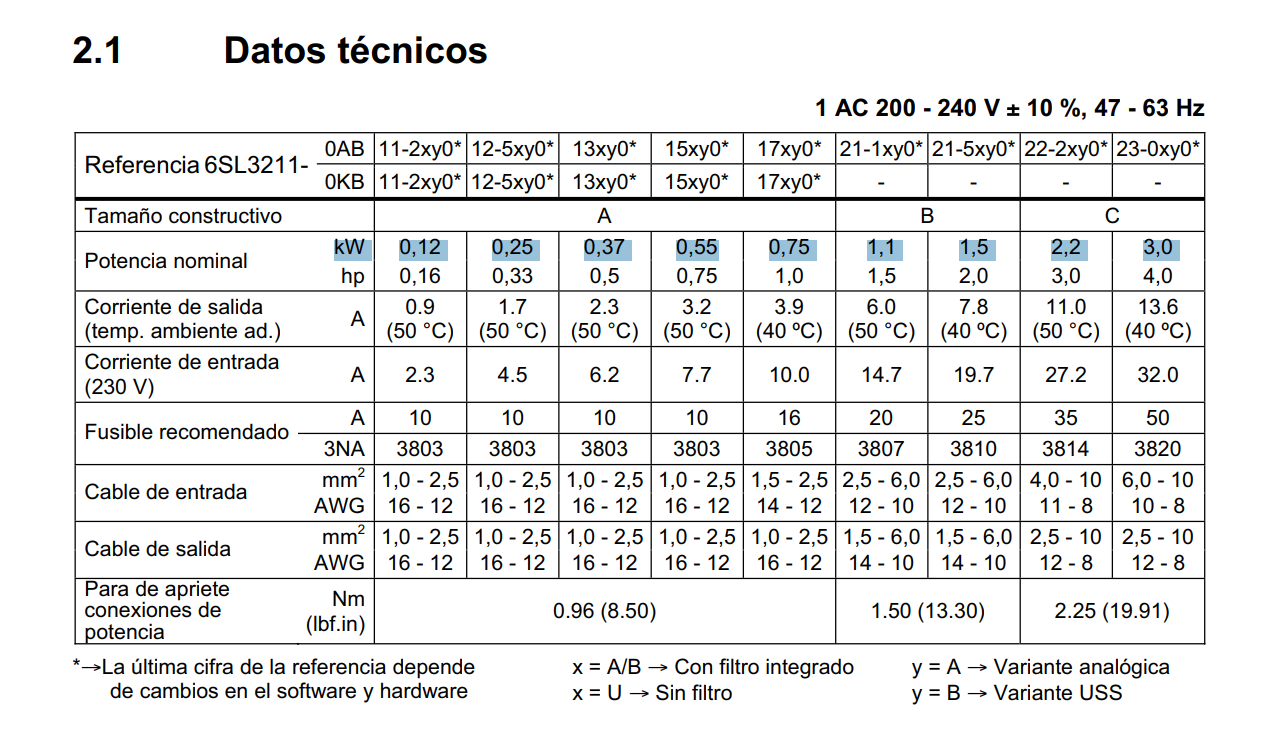
\includegraphics[width=1\linewidth]{Figura 3.png}        \caption{\href{https://cache.industry.siemens.com/dl/files/910/20976910/att_109514/v1/G110_COM_1104_20976910_SP.pdf}{Hoja de Datos del Sinamics 110}. [6]}
        \label{fig:fig_3}
    \end{figure}

    Se observa en la \autoref{fig:fig_3}, remarcado de color celeste que el rango de potencias es de $0.12 \ [kW]$ hasta los $3.0 \ [kW]$ de acuerdo al tamaño constructivo del variador (A, B o C).


    \item \underline{Tipo de Control de Velocidad:} Dado que un variador de frecuencia busca generar un arranque suave modificando de forma controlada la tensión y frecuencia de alimentación del motor, se tiene que para este variador, el fabricante provee los siguientes pasos para ajustar y definir el control de velocidad:
    \begin{figure}[H]
        \centering
        
\includegraphics[width=1\linewidth]{Figura 4.png}        \caption{\href{https://cache.industry.siemens.com/dl/files/910/20976910/att_109514/v1/G110_COM_1104_20976910_SP.pdf}{Hoja de Datos del Sinamics 110}. [6]}
        \label{fig:fig_4}
    \end{figure}
    \begin{figure}[H]
        \centering
        
\includegraphics[width=1\linewidth]{Figura 5.png}        \caption{\href{https://cache.industry.siemens.com/dl/files/910/20976910/att_109514/v1/G110_COM_1104_20976910_SP.pdf}{Hoja de Datos del Sinamics 110}. [6]}
        \label{fig:fig_5}
    \end{figure}

    Como se observa en la documentación presentada por el fabricante según la \autoref{fig:fig_4} y la \autoref{fig:fig_5}, el modo de regulación principal se selecciona con el parámetro $P1300$. Adicionalmente, el fabricante ilustra cómo el control $\frac{V}{f}$ permite configurar una elevación de tensión (Boost) continua o de aceleración mediante los parámetros P1310 y P1311. Esta función es de suma importancia en el control escalar, ya que a bajas frecuencias, la caída de tensión en la resistencia del estator impide mantener el flujo magnético constante. La función 'Boost' compensa esta caída inyectando un porcentaje de tensión adicional, garantizando así que el motor disponga del par necesario para su correcto funcionamiento.
    
    
    \item \underline{Diagrama en Bloque del Variador:} El fabricante presenta de forma directa el diagrama en bloques tal como muestra la \autoref{fig:fig_6}.
    \begin{figure}[H]
        \centering
        
\includegraphics[width=0.8\linewidth]{Figura 6.png}        \caption{\href{https://cache.industry.siemens.com/dl/files/910/20976910/att_109514/v1/G110_COM_1104_20976910_SP.pdf}{Hoja de Datos del Sinamics 110}. [6]}
        \label{fig:fig_6}
    \end{figure}


    \item \underline{Borneras de Conexión y Circuito de Potencia y Control:} El fabricante entrega dentro de su hoja de datos un esquemático planteado para los circuitos de potencia y de control los cuales se presentan en la \autoref{fig:fig_7}.
    \begin{figure}[H]
        \centering
        
\includegraphics[width=0.8\linewidth]{Figura 7.png}        \caption{\href{https://cache.industry.siemens.com/dl/files/910/20976910/att_109514/v1/G110_COM_1104_20976910_SP.pdf}{Hoja de Datos del Sinamics 110}. [6]}
        \label{fig:fig_7}
    \end{figure}
    
    El equipo cuenta con terminales divididos según su propósito. Asumiendo la versión estándar con entradas analógicas, el esquema para el circuito de potencia es el siguiente:
    \begin{itemize}
        \item \underline{L1 y L2/N:} Bornes para la alimentación desde la red monofásica externa.
        \item \underline{PE:} Borne para la conexión de protección de puesta a tierra.
        \item \underline{U, V, W:} Bornes de salida trifásica de potencia hacia las borneras del motor.
    \end{itemize}
    
    En cuanto al circuito de control, la configuración con potenciómetro y pulsadores es la siguiente:
    \begin{itemize}
        \item \underline{Borne 3 ($DIN0$):} Entrada digital configurada de fábrica ($P0701 = 1$) para la orden de Marcha ($ON$) / Paro ($OFF1$).
        \item \underline{Borne 4 ($DIN1$):} Entrada digital configurada ($P0702 = 12$) para la orden de Inversión de giro.
        \item \underline{Borne 5 ($DIN2$):} Entrada digital configurada ($P0703 = 9$) para el Acuse de fallo ($Reset$).
        \item \underline{Conexión del Potenciómetro:} Se utilizan tres bornes. El borne 8 entrega la tensión de referencia ($+ 10 \ [V]$), el borne 10 es la masa ($0 \ [V]$), y el cursor central del potenciómetro se conecta al borne 9 ($AIN+$), entregando una señal analógica proporcional ($0$ a $10 \ [V]$) que el equipo traduce en la consigna de velocidad.
    \end{itemize}


    \item \underline{Diagrama de flujo para la puesta en servicio y parámetros importantes:} El diagrama de bloques para la "Puesta en servicio rápida" que debe seguir el operador consta de los siguientes pasos consecutivos:
    \begin{figure}[H]
        \centering
        
\includegraphics[width=1\linewidth]{Figura 8.png}        \caption{\href{https://cache.industry.siemens.com/dl/files/910/20976910/att_109514/v1/G110_COM_1104_20976910_SP.pdf}{Hoja de Datos del Sinamics 110}. [6]}
        \label{fig:fig_8}
    \end{figure}
    \begin{figure}[H]
        \centering
        
\includegraphics[width=1\linewidth]{Figura 9.png}        \caption{\href{https://cache.industry.siemens.com/dl/files/910/20976910/att_109514/v1/G110_COM_1104_20976910_SP.pdf}{Hoja de Datos del Sinamics 110}. [6]}
        \label{fig:fig_9}
    \end{figure}
    \begin{figure}[H]
        \centering
        
\includegraphics[width=1\linewidth]{Figura 10.png}        \caption{\href{https://cache.industry.siemens.com/dl/files/910/20976910/att_109514/v1/G110_COM_1104_20976910_SP.pdf}{Hoja de Datos del Sinamics 110}. [6]}
        \label{fig:fig_10}
    \end{figure}

    Si bien a lo largo de la \autoref{fig:fig_8}, \autoref{fig:fig_9} y \autoref{fig:fig_10} se ha destacado el paso a paso de la puesta en servicio, se lista brevemente a continuación una lista de los parámetros más importantes:
    \begin{itemize}
        \item \underline{$P0304$ a $P0310$:} Son los parámetros obligatorios donde se introduce toda la información de la chapa del motor (En síntesis, todos los parámetros vistos para la \autoref{fig:fig_1} si quisiéramos controlar tal motor).
        \item \underline{$P0700$:} Define la fuente de las órdenes de marcha y paro (Ajustar en 2 para control por bornes).
        \item \underline{$P1000$:} Define la fuente de la consigna de velocidad (Ajustar en 2 para usar el potenciómetro analógico).
        \item \underline{$P1080 / P1082$:} Frecuencia mínima y máxima del motor (por ejemplo de $0 \ [Hz]$ a $50 \ [Hz]$).
        \item \underline{$P1120 / P1121$:} Se definen los tiempos de aceleración y deceleración en segundos.
        \item \underline{$P1300$:} Define el modo de control, por defecto 0 ($\frac{V}{f}$ lineal).
    \end{itemize}
\end{itemize}



\subsubsection{Conclusiones Parciales}
A lo largo de los últimos Trabajos Prácticos, hemos visto como implementar el control de motores de forma indirecta mediante la rectificación semi o totalmente controlada, o mediante el uso de drivers para motores de CC. Sin embargo para los motores de CA, el análisis es distinto ya que el modelo del motor es otro.

En este trabajo, vimos que el variador SINAMICS G110 permite comprender los alcances y las limitaciones prácticas de los convertidores de frecuencia de gama básica. A través del estudio de su hoja de datos, se constató que el control escalar $V/f$ lineal o cuadrático es una solución sumamente eficiente y económica para aplicaciones industriales de baja exigencia dinámica, donde funciones como la elevación de tensión (Boost) resultan críticas para mantener el flujo magnético constante y evitar la pérdida de par a bajas revoluciones.

A modo de conclusión general (y de forma complementaria para unificar el análisis de ambas consignas), se concluye que no es posible integrar el motor de CA analizado en la primera etapa de este Trabajo Práctico con el variador de Siemens recién visto. Esto se debe a que el rango de potencia nominal que ofrece la gama G110 de Siemens se limita a tan solo $3.0 \ [kW]$ (para su tamaño constructivo C), lo cual resulta completamente incompatible e insuficiente para comandar un motor de $7.5 \ [kW]$. Este hallazgo resalta una conclusión fundamental en el diseño de circuitos de electrónica de potencia analizados a lo largo de estos 10 Trabajos Prácticos: \textit{Es fundamental conocer el funcionamiento tanto de los dispositivos de control como de los de potencia, ya que un entendimiento deficiente de estos componentes provoca una falta de coordinación entre sus valores característicos, lo que puede derivar en daños graves y de un alto costo económico para los equipos.}



\section{Bibliografía}
\begin{itemize}
    \raggedright
    \item \underline{$[1]$:} Power Systems International. (s.f.). \textit{Guide to international power frequencies} [Guía técnica]. \url{https://powersystemsinternational.com/guide-to-international-power-frequencies/}

    \item \underline{$[2]$:} Agüero, A. (2017). \textit{Control de motores de corriente alterna} (p. 22-25) [Apunte de cátedra]. Cátedra de Electrónica Industrial, Departamento de Electrónica, F.C.E.F. y N., Universidad Nacional de Córdoba. \url{https://efn.unc.edu.ar/}

    \item \underline{$[3]$:} Calcuvio. (s.f.). \textit{Convertir radianes por segundo a rpm} [Plataforma de cálculo en línea]. \url{https://www.calcuvio.com/radianes-segundo-rpm}

    \item \underline{$[4]$:} SB Argentina. (s.f.). \textit{Motor eléctrico trifásico MT 132S2-2 10HP 2 polos 380/660} [Ficha de producto en línea]. \url{https://www.sbargentina.com.ar/tienda/MOTOR-ELECTRICO-TRIFASICO-MT-132S2-2-10HP-2-POLOS-380-660}

    \item \underline{$[5]$:} International Electrotechnical Commission. (2022). \textit{IEC 60072-1:2022. Rotating electrical machines - Dimensions and output series - Part 1: Frame numbers 56 to 400 and flange numbers 55 to 1080} [Norma internacional]. \url{https://webstore.iec.ch/en/publication/67088}

    \item \underline{$[6]$:} Siemens. (2004). \textit{SINAMICS G110: Manual de instrucciones de operación} [Manual técnico]. \url{https://cache.industry.siemens.com/dl/files/910/20976910/att_109514/v1/G110_COM_1104_20976910_SP.pdf}
    
\end{itemize}
\end{document}